% Especificaciones del tamaño de letra, tamaño de hoja, márgenes, librerias, etc.
\documentclass[12pt, letterpaper]{article}
\usepackage[english]{babel}
\usepackage{fancyhdr}
\usepackage[utf8]{inputenc}
\usepackage[T1]{fontenc}
\usepackage{amsmath}
\usepackage{graphicx}
\usepackage{subcaption}
\usepackage[hidelinks]{hyperref}
\usepackage{url}
\usepackage{amssymb}
\usepackage{float}
\usepackage[margin=1in]{geometry}
\usepackage[framed, numbered]{matlab-prettifier}
\renewcommand{\baselinestretch}{1.5}

% Enlace Bibliografía
\usepackage{csquotes}
\usepackage[notes,backend=biber]{biblatex-chicago}
\addbibresource{referencias.bib}

% Titulo, autores, fecha.
\title{Práctica \#4: Acciones Básica de Control y Respuesta de Sistemas de Control}
\author{Carlos Vásquez \and 1155057}
\date{May 29, 2019}
\pagestyle{fancy}
\fancyhf{}
\rhead{Carlos Vásquez}
\lhead{Práctica \#4}
\rfoot{\thepage}


% Inicio del documento
\begin{document}
\maketitle
\section*{Introducción}

Los sistemas de control son útiles para lograr llevar la señal de un sistema a un valor deseado y asì obtener el comportamiento que requerimos de una planta especificada. Entre los sistemas de control básicos se encuentran el controlador proporcional, el proporcional-integral, el proporcional-integral-derivativo, entre otros, los cuales son muy sencillos de implementar y ampliamente utilizados y comprendidos entre ingenieros de control. Estos controladores terminan reducièndose a un manipulamiento de la señal de entrada bastante básico y sólo requieren especificar valores de las ganancias de control.

La mayoría de los casos cuando se implementan este tipo de controladores será necesario, mediante prueba y error, darle valor a estas constantes y lograr estabilizar nuestro sistema al nivel de referencia que hemos establecido con anterioridad. A lo largo del desarrollo de la práctica observaremos las distintas ventajas y desventajas con las que cuentan estos controladores en particular.

\section*{Desarrollo}

\begin{enumerate}
	\item Para la figura mostrada a continuación:
		\begin{figure}[H]
			\centering
			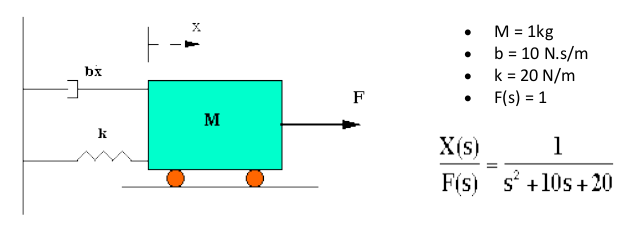
\includegraphics[width=0.8\textwidth]{planta.png}
			\caption{Esquema del sistema dinámico a analizar.}
		\end{figure}
		\begin{enumerate}
			\item Ingrese la función de transferencia en MATLAB y obtenga la respuesta a escalón en lazo abierto.

				Como se muestra en la imagen, la función te transferencia de nuestra planta es
				\begin{equation}
					\frac{X(s)}{F(s)} + \frac{1}{s^2 + 10s + 20}
				\end{equation}
				Por lo tanto, simplemente tenemos que abrir un bloque de función de transferencia en MATLAB con una entrada escalón unitario con valor de 1, como se muestra en la figura 2.
				\begin{figure}[H]
					\centering
					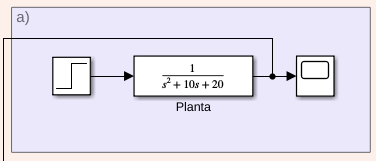
\includegraphics[width=0.5\textwidth]{1a.png}
					\caption{Diagrama de bloques para el (a).}
				\end{figure}
				\begin{figure}[H]
					\centering
					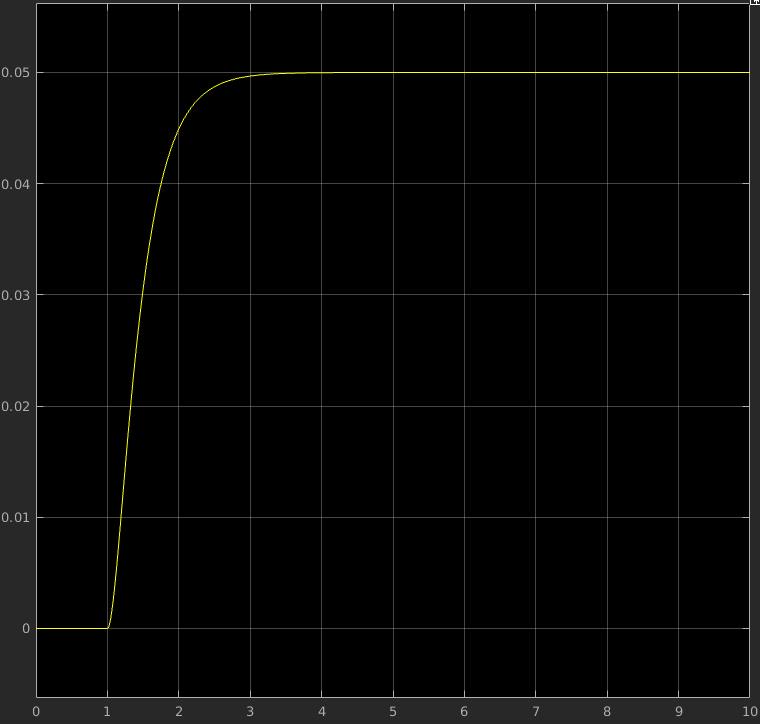
\includegraphics[width=0.7\textwidth]{1aa.png}
					\caption{Gráfica de la respuesta obtenida para (a).}
				\end{figure}
			
			\item Ingrese ahora un controlador proporcional para lazo cerrado con valor $K_p = 300$. Obtenga la respuesta a escalón en lazo cerrado (Control P).

				La función de transferencia para esta planta en específico con este controlador será la siguiente.
				\begin{equation}
					\frac{X(s)}{F(s)} = \frac{K_p}{s^2 + 10s + (20 + K_p)}
				\end{equation}
				Una vez reemplazado el valor de $K_p =  300$ a nuestra planta obtendremos la siguiente función de transferencia.
				\begin{equation}
					\frac{X(s)}{F(s)} = \frac{300}{s^2 + 10s + 320}
				\end{equation}
				\begin{figure}[H]
					\centering
					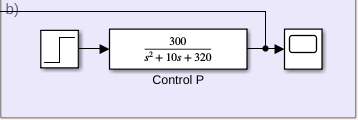
\includegraphics[width=0.5\textwidth]{1b.png}
					\caption{Diagrama de bloques para (b).}
				\end{figure}

				\begin{figure}[H]
					\centering
					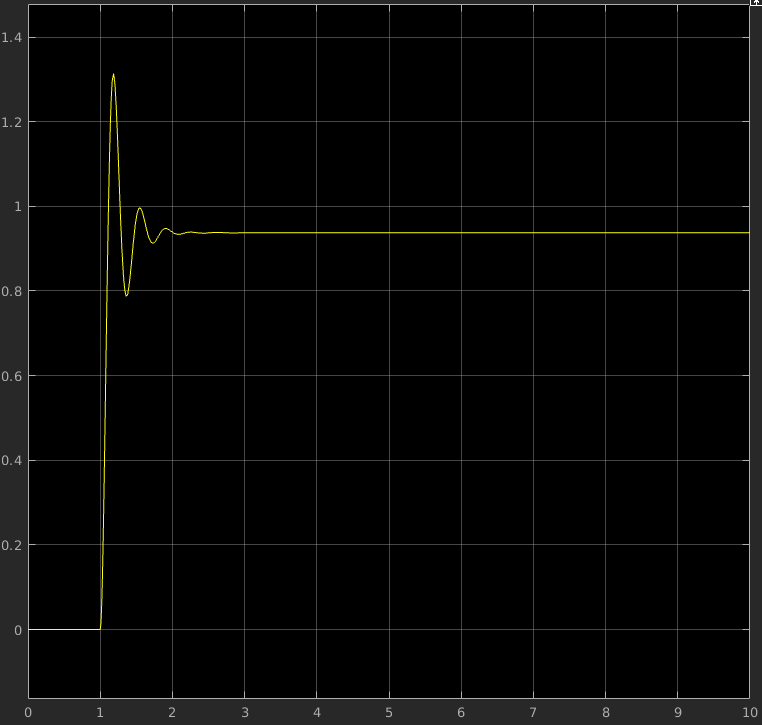
\includegraphics[width=0.6\textwidth]{1bb.png}
					\caption{Gráfica de la respuesta obtenida para (b).}
				\end{figure}
			
			\item Añada un controlador derivativo de valor $K_d = 10$. Obtenga la respuesta escalón en lazo cerrado (Control PD).

				La función de transferencia para la planta junto con este controlador PD será la siguiente:
				\begin{equation}
					\frac{X(s)}{F(s)} = \frac{K_ds + K_p}{s^2 + (10 + K_p) + (20 + K_p)}
				\end{equation}
				Con esta función y sustituyendo los valores dados obtenemos la función:
				\begin{equation}
					\frac{X(s)}{F(s)} = \frac{10s + 300}{s^2 + 310s + 320}
				\end{equation}
				\begin{figure}[H]
					\centering
					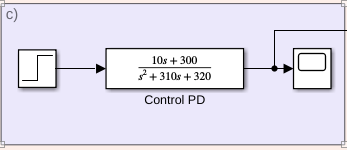
\includegraphics[width=0.5\textwidth]{1c.png}
					\caption{Diagrama de bloques para (c).}
				\end{figure}

				\begin{figure}[H]
					\centering
					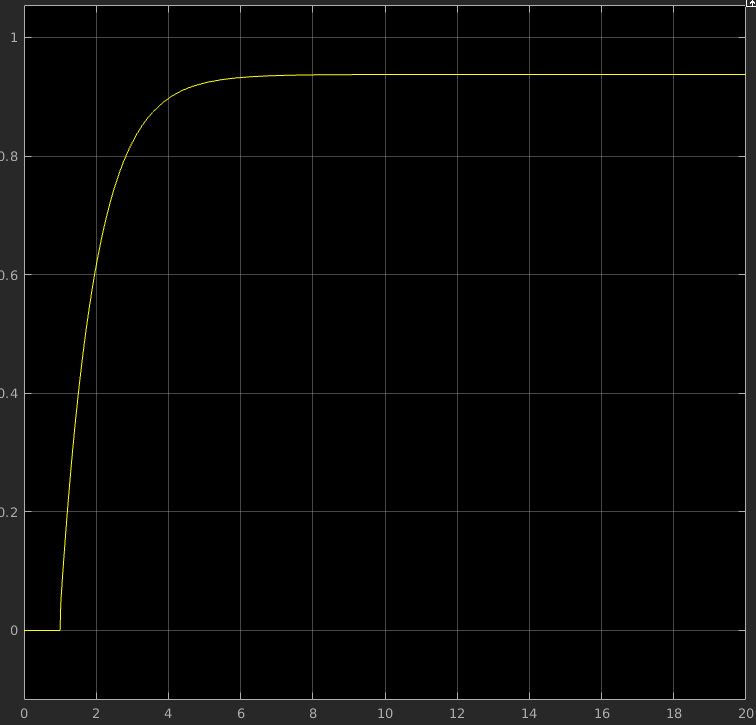
\includegraphics[width=0.6\textwidth]{1cc.png}
					\caption{Gráfica de la respuesta obtenida  para (c).}
				\end{figure}
				
			\item Utilice un controlador proporcional de valor $K_p = 30$ y uno integral de valor $K_i = 70$. Obtenga la respuesta escalón en lazo cerrado (Control PI).
				
				Como hemos visto antesm la función de transferencia para este tipo de controlador quedará de la siguiente manera.
				\begin{equation}
					\frac{X(s)}{F(s)} = \frac{K_ps + K_i}{s^3 + 10s^2 + (20 + K_p)s + K_i}
				\end{equation}
				Y sustituyendo los valores que nos indica la práctica obtendremos la siguiente función:
				\begin{equation}
					\frac{X(s)}{F(s)} = \frac{30s + 70}{s^3 + 10s^2 + 50s + 70}
				\end{equation}
				
				\begin{figure}[H]
					\centering
					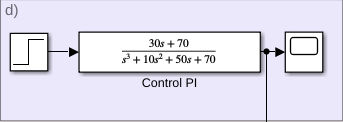
\includegraphics[width=0.5\textwidth]{1d.png}
					\caption{Diagrama de bloques para (d).}
				\end{figure}
				
				\begin{figure}[H]
					\centering
					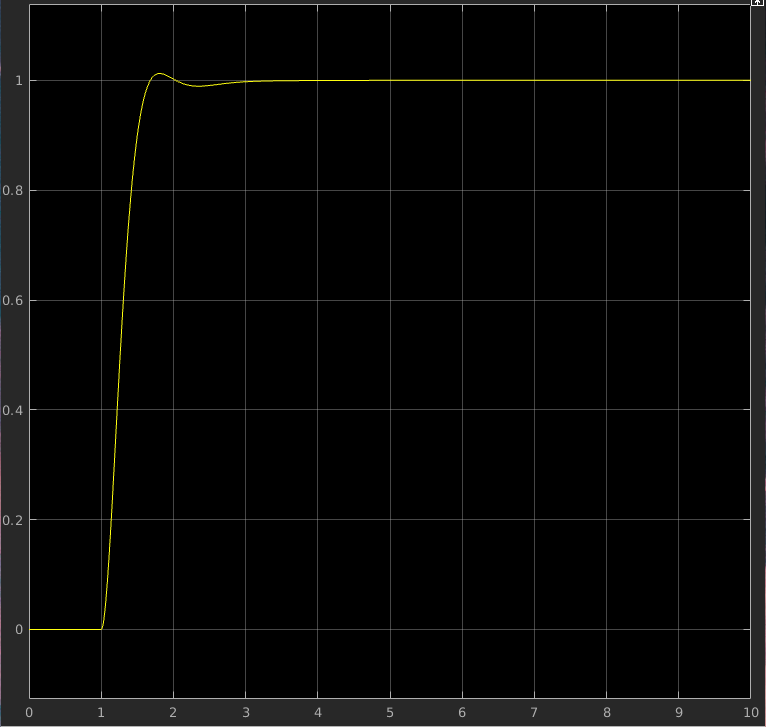
\includegraphics[width=0.6\textwidth]{1dd.png}
					\caption{Gráfica de la respuesta obtenida para (d).}
				\end{figure}

			\item Utilice un controlador proporcional de valor $K_p = 350$, uno integral de valor $K_i = 300$ y un controlador derivativo $K_d = 50$. Obtenga la respuesta escalón en lazo cerrado (Control PID).

				La función de transferencia para esta planta implementada con este controlador será
				\begin{equation}
					\frac{X(s)}{F(s)} = \frac{K_ds^2 + K_ps + K_i}{s^3 + (10 K_d)s^2 + (20 + K_p)s + K_i}
				\end{equation}
				Y una vez sustituidos los valores dados, obtenemos la función de transferencia para el controlador y planta específica con la cual contamos.
				\begin{equation}
					\frac{X(s)}{F(s)} = \frac{50s^2 + 350s + 300}{s^3 + 60s^2 + 370s + 300}
				\end{equation}

				\begin{figure}[H]
					\centering
					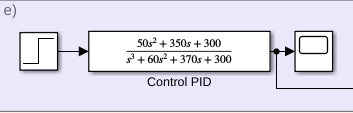
\includegraphics[width=0.5\textwidth]{1e.png}
					\caption{Diagrama de bloques para (e).}
				\end{figure}

				\begin{figure}[H]
					\centering
					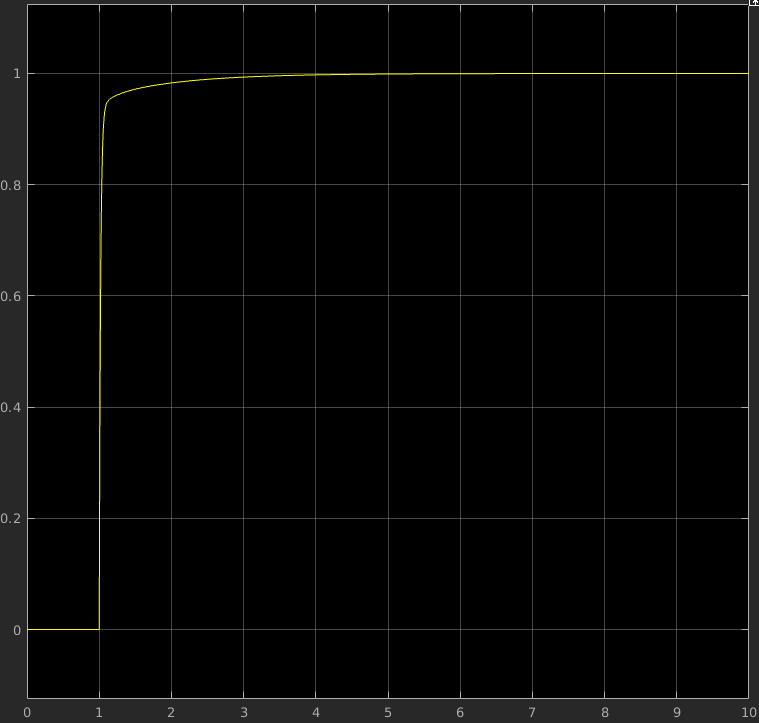
\includegraphics[width=0.6\textwidth]{1ee.png}
					\caption{Gráfiica de la respuesta obtenida para (e).}
				\end{figure}

				Si comparamos todas las respuestas obtenidas tendremos una apreciación más amplia de cómo los distintos controladores actúan y cuáles son más efectivos.
				
				\begin{figure}[H]
					\centering
					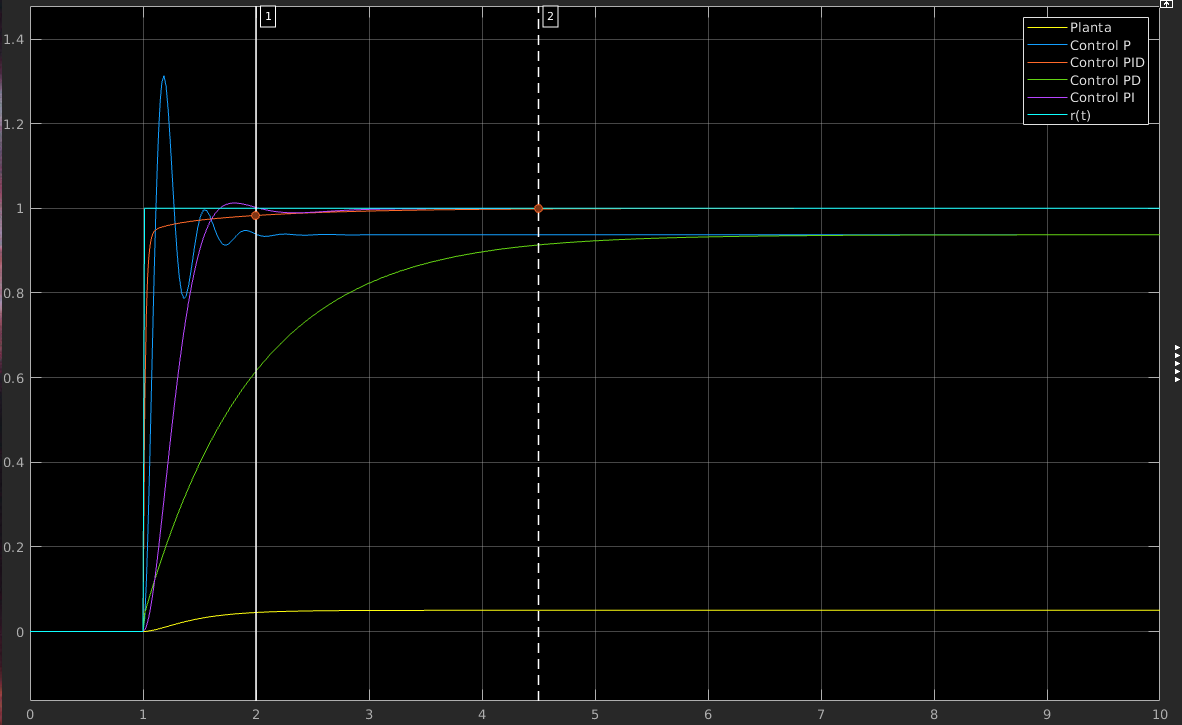
\includegraphics[width=\textwidth]{1t.png}
					\caption{Gráfica de los distinos controladores, planta y la señal de referencia.}
				\end{figure}
				\textit{¿Cuáles son las diferencias principales que observa con cada controlador?}

				Los controladores actúan de manera distinta, unos se estabilizan en un tiempo más corto, sin embargo puede que tarden más en llegar al nivel de referencia que es deseado, o que no alcancen este nivel en lo absoluto. Otros tienen un sobre impulso, superando el nivel de referencia y propagando este sobre impulso a través de la respuesta estable del sistema.

				\textit{¿Qué método resulta más conveniente para mejorar el sobreimpulso?}

				El controlador PID resulta muy eficaz mejorando este sobreimpulso. Debido a su parte integradora, el sobre impulso que tiene el controlador proporcional integral es inevitable, sin embargo, el controlador proporcional diferencial atenua este sobreimpulso, y si los combinamos obtenemos un controlador que nos combina estas dos características y elimina gran parte del error.

				\textit{¿Con qué controlador se mejora el tiempo de crecimiento?}

				Observando la figura 12, podemos decir con certeza que el controlador PID es el que obtiene el menor tiempo de crecimiento para esta planta.

		\end{enumerate}

	\item Crear en SIMULINK las diferentes acciones de control para la siguiente planta.

				\begin{figure}[H]
					\centering
					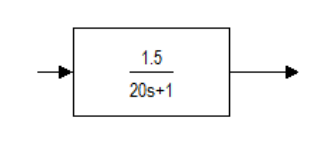
\includegraphics[width=0.4\textwidth]{planta2.png}
				\end{figure}
				\begin{enumerate}
					\item Controlador On-Off

						Este controlador es un simple \textit{relay}, el cual se activará para que nuestra planta alcance el nivel de referencia deseado, que en este caso es 20.

				\begin{figure}[H]
					\centering
					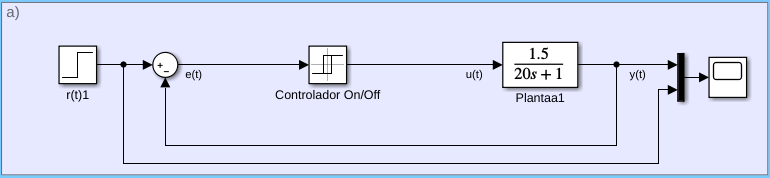
\includegraphics[width=0.7\textwidth]{2a.png}
					\caption{Diagrama de bloques para el controlador on-off.}
				\end{figure}

				\begin{figure}[H]
					\centering
					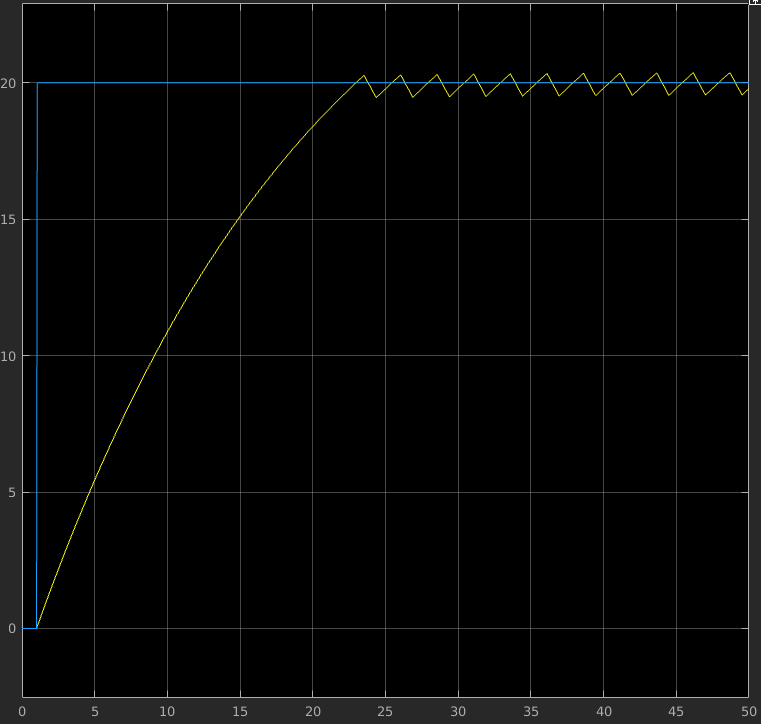
\includegraphics[width=0.5\textwidth]{2aa.png}
					\caption{Gráfica del comportamiento del controlador on-off.}
				\end{figure}
					\item Controlador Proporcional
						
						El controlador proporcional, como su nombre lo dice, utiliza una constante de proporcionalidad, la cual es la ganancia del controlador y es muy sencilla de implementar.

				\begin{figure}[H]
					\centering
					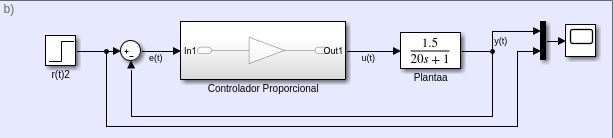
\includegraphics[width=0.5\textwidth]{2b.png}
					\caption{Diagrama de bloques para el controlador proporcional.}
				\end{figure}

				\begin{figure}[H]
					\centering
					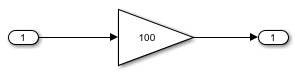
\includegraphics[width=0.5\textwidth]{2bb.png}
					\caption{Diagrama de bloques para el subsistema que representa el controlador proporcional.}
				\end{figure}

				\begin{figure}[H]
					\centering
					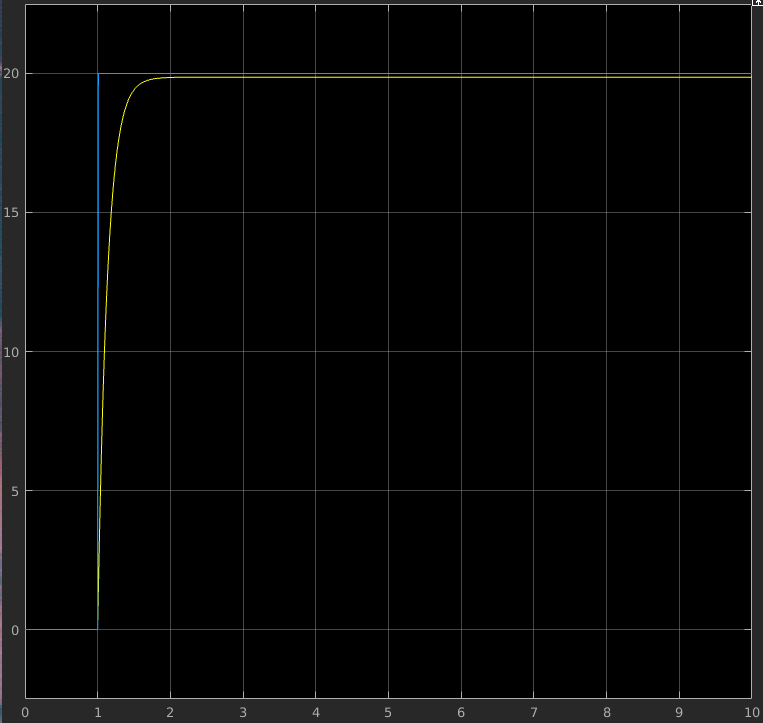
\includegraphics[width=0.5\textwidth]{2bbb.png}
					\caption{Gráfica del comportamiento del controlador proporcional.}
				\end{figure}

					\item Controlador Integral

						Para este controlador obtenemos lo siguiente.

				\begin{figure}[H]
					\centering
					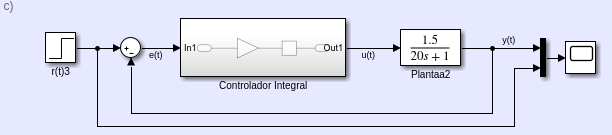
\includegraphics[width=0.5\textwidth]{2c.png}
					\caption{Diagrama de bloques para el controlador integral.}
				\end{figure}

				\begin{figure}[H]
					\centering
					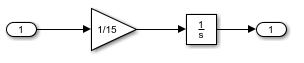
\includegraphics[width=0.5\textwidth]{2cc.png}
					\caption{Diagrama de bloques el subsistema que es el controlador.}
				\end{figure}

				\begin{figure}[H]
					\centering
					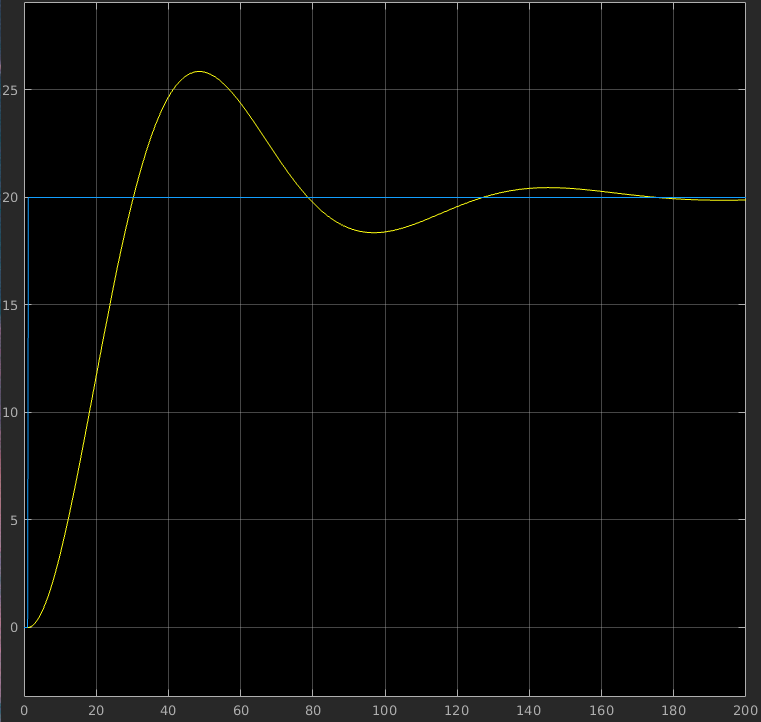
\includegraphics[width=0.5\textwidth]{2ccc.png}
					\caption{Respuesta del controlador contra la referencia dada.}
				\end{figure}
						Como es posible apreciarlo en las figuras anteriores, el controlador integral por su cuenta es muy lento y su sobreimpulso es bastante amplio.
					\item Controlador Proporcional-Integral

						Este controlador combina las características del controlador proporcional y el integral, obteniendo una atenuación de impulso, sin embargo el valor de referencia no es alcanzado por el controlador.

				\begin{figure}[H]
					\centering
					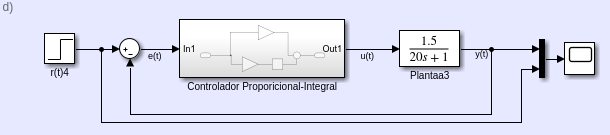
\includegraphics[width=0.5\textwidth]{2d.png}
					\caption{Diagrama de bloques para el controlador proporcional-integral.}
				\end{figure}

				\begin{figure}[H]
					\centering
					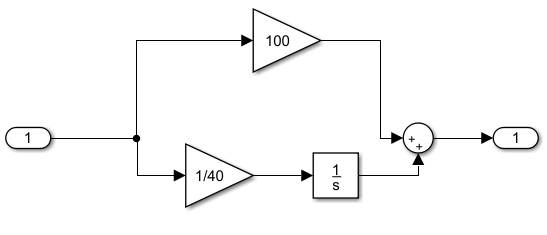
\includegraphics[width=0.5\textwidth]{2dd.png}
					\caption{Diagrama de bloques para el subsistema que es el controlador PI.}
				\end{figure}
				
				\begin{figure}[H]
					\centering
					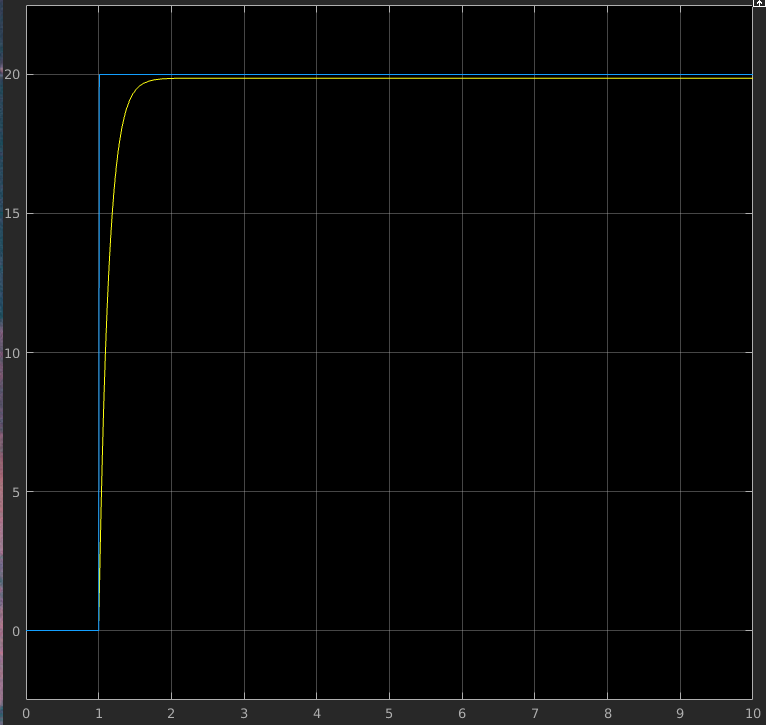
\includegraphics[width=0.5\textwidth]{2ddd.png}
					\caption{Respuesta del controlador.}
				\end{figure}
					\item Controlador Derivativo

						Como hemos visto teóricamente, este controlador por sí sólo no es capaz de controlar la señal debido a que los cambios en referencia son de tipo escalón. Sólo reacciona cuando hay cambio en el error. Su función es más trabajar como controlador predictor, lo cual nos ayuda a eliminar el sobreimpulso en otros controladores. Sin embargo si existe ruido en la señal, este controlador sólo lo amplifica.
				\begin{figure}[H]
					\centering
					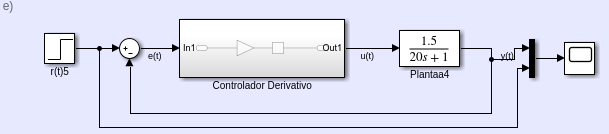
\includegraphics[width=0.5\textwidth]{2e.png}
					\caption{Diagrama de bloques para el controlador derivativo.}
				\end{figure}
				
				\begin{figure}[H]
					\centering
					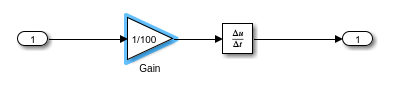
\includegraphics[width=0.5\textwidth]{2ee.png}
					\caption{Diagrama de bloques para el subsistema que es el controlador.}
				\end{figure}

				\begin{figure}[H]
					\centering
					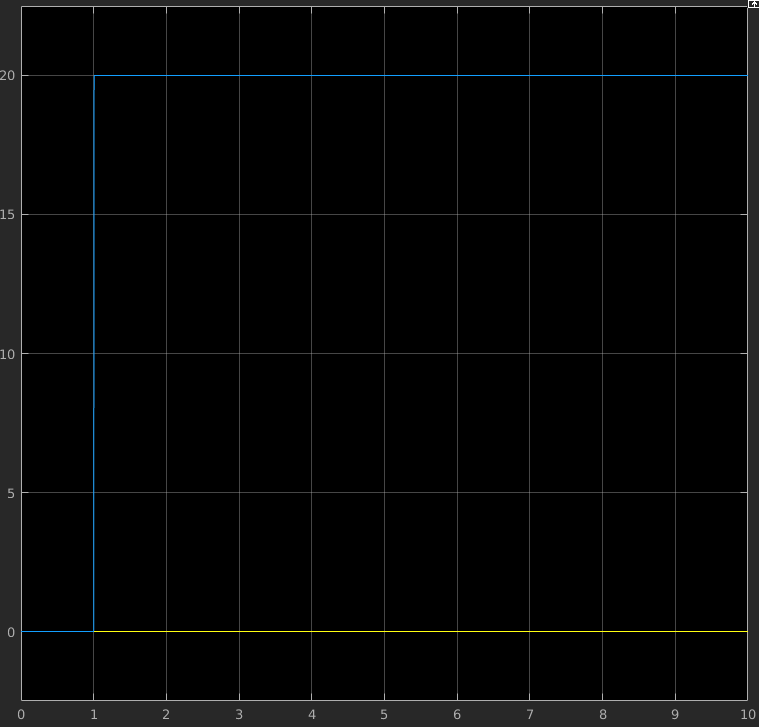
\includegraphics[width=0.5\textwidth]{2eee.png}
					\caption{Respuesta del controlador.}
				\end{figure}

					\item Controlador Proporcional-Derivativo
						Este controlador ya es capaz de controlar la señal, a diferencia del anterior. El sobreimpulso será mínimo, sino es que nulo, pero no se logrará eliminar el error tan efectivamente en el estado estable.

				\begin{figure}[H]
					\centering
					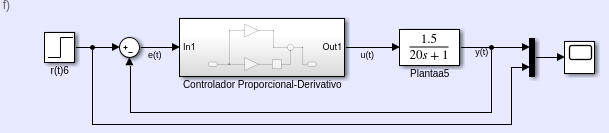
\includegraphics[width=0.5\textwidth]{2f.png}
					\caption{Diagrama de bloques para el controlador proporcional-derivativo.}
				\end{figure}
				
				\begin{figure}[H]
					\centering
					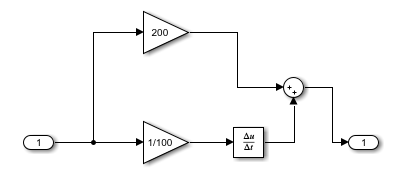
\includegraphics[width=0.5\textwidth]{2ff.png}
					\caption{Diagrama de bloques para el subsistema que es el controlador.}
				\end{figure}

				\begin{figure}[H]
					\centering
					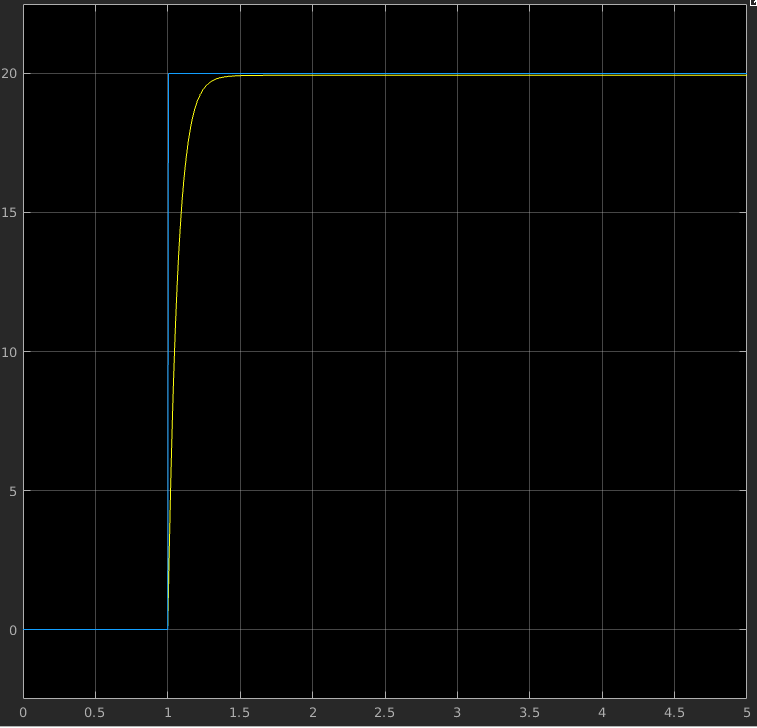
\includegraphics[width=0.5\textwidth]{2fff.png}
					\caption{Respuesta del controlador.}
				\end{figure}
				\end{enumerate}

			\item Para los siguiente polinomios característicos, grafique con MATLAB los polos y ceros utilizando el comando \textit{pzmap(G)}. COnsidere una ganancia de numerador $K = 2$. Indique si es un sistema estable o inestable de acuerdo al criterio de estabilidad de Routh.
				\begin{enumerate}
					\item $s^3 - 2s^2 - 5s + 6$
					\item $s^4 + 7s^3 + 24s^2 + 58s + 40$
					\item $s^6 + 5s^5 + 6s^4 + 10s^3 + 4s + 1$
				\end{enumerate}
				El código utilizado en matlab es el siguiente.
				\lstinputlisting[style=Matlab-editor, basicstyle=\mlttfamily\scriptsize, caption = {Código para graficar los polos y ceros de los polinomios.}]{./code/3.m}

				\begin{figure}[H]
					\centering
					\begin{subfigure}[b]{0.49\linewidth}
						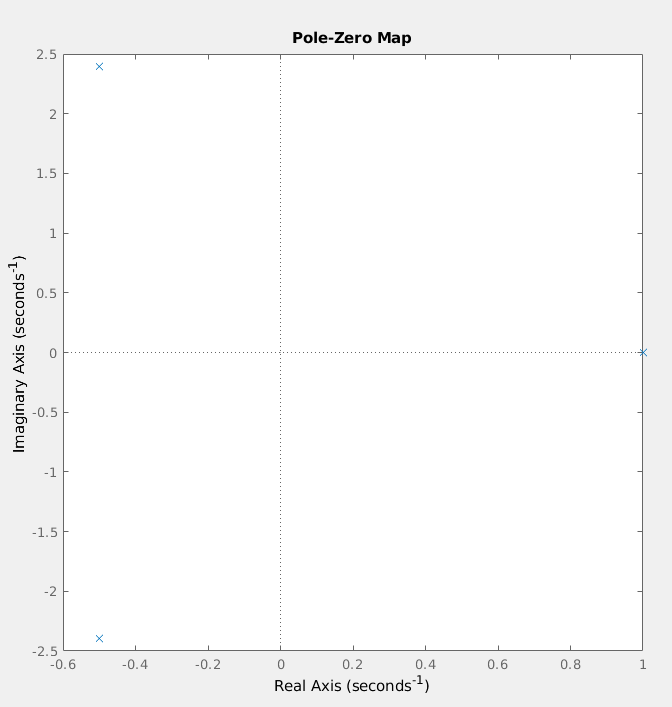
\includegraphics[width=\linewidth]{3a.png}
						\caption{El primer polinomio no es estable dado que el comportamiento exponencial de este sistema aumenta, ya que uno de sus polos, su parte real es mayor a cero.}
					\end{subfigure}
					\begin{subfigure}[b]{0.49\linewidth}
						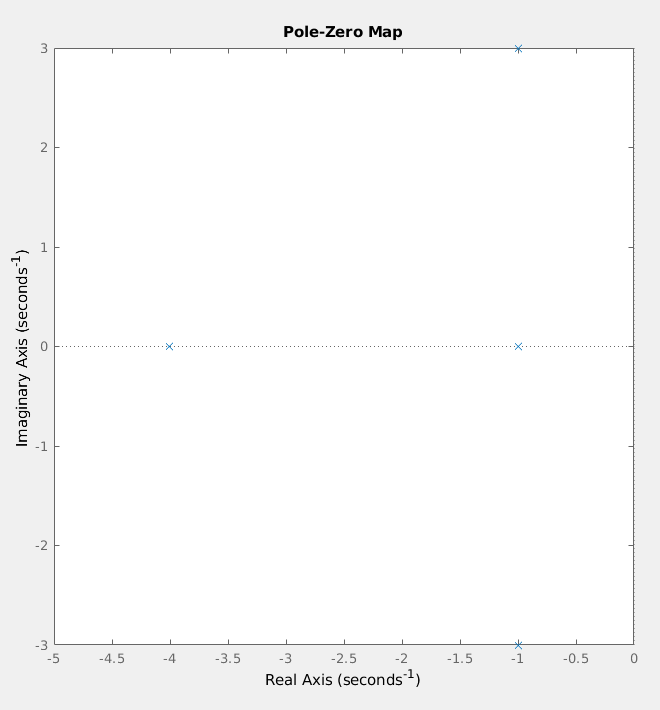
\includegraphics[width=\linewidth]{3b.png}
						\caption{Este polinomio sí es estable dado que todos sus polos se encuentran donde $Re < 0$, por lo que su transitorio se desvanece a lo largo del tiempo.}
					\end{subfigure}
					\begin{subfigure}[b]{0.49\linewidth}
						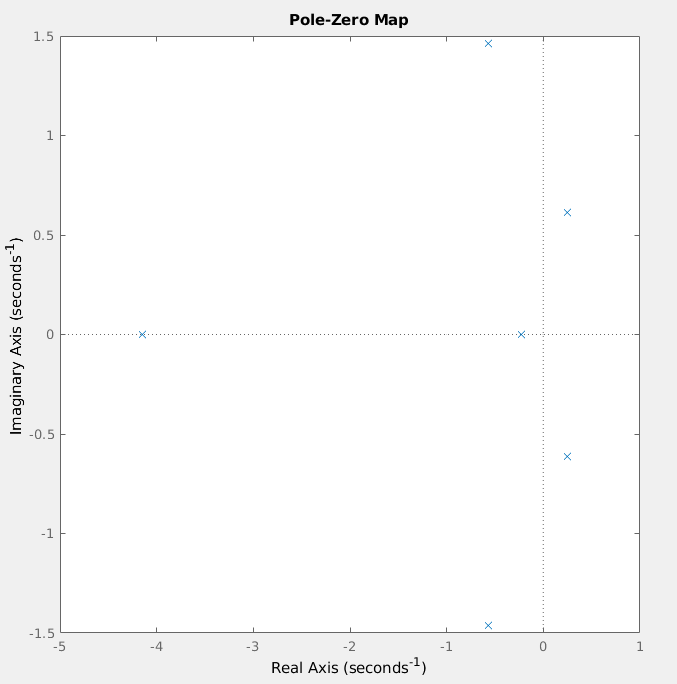
\includegraphics[width=\linewidth]{3c.png}
						\caption{Al igual que (a),el transitorio no se elimina a lo largo del tiempo.}
					\end{subfigure}
					\caption{Gráficas de los polinomios y sus raíces en el plano complejo.}
				\end{figure}
			
			\item Para los siguientes polinomios característicos, grafique con MATLAB los polos  y ceros utilizando el comando \textit{pzmap(G)}. Considere una ganancia de numerador de K = 2. Indique si es un sistema estable o inestable de acuerdo al criterio de Routh.
				\begin{enumerate}
					\item $\frac{K(s+1)}{(s-2)(s+1)}$
					\item $\frac{K}{(s-1)(s+5)(s+20)}$
					\item $\frac{K(s+1)}{(s-1)(s-2)}$
				\end{enumerate}
				Al igual que el ejercicio anterior, se desarrolló el siguiente código en MATLAB.
				\lstinputlisting[style=Matlab-editor, basicstyle=\mlttfamily\scriptsize, caption = {Código para graficar los polos y ceros de los polinomios.}]{./code/4.m}
				Y los resultados de las gráficas se muestran a continuación.
				\begin{figure}[H]
					\centering
					\begin{subfigure}[b]{0.49\linewidth}
						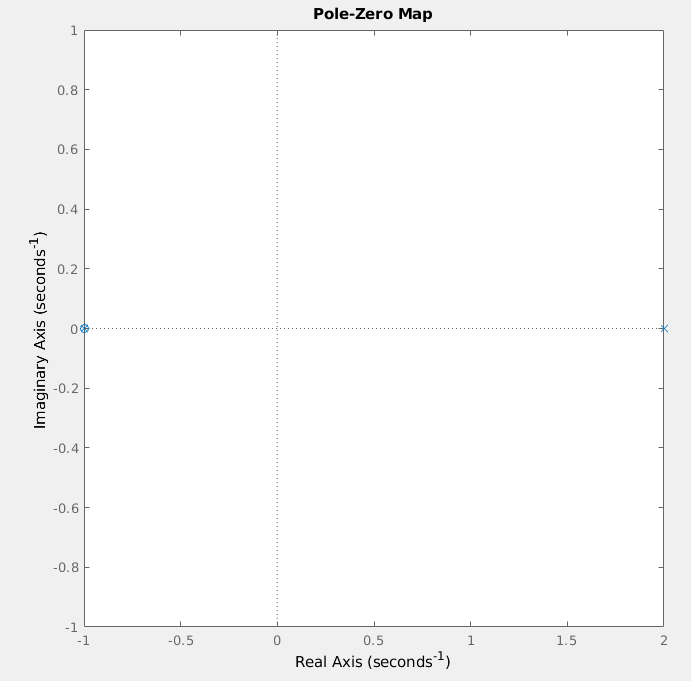
\includegraphics[width=\linewidth]{4a.png}
						\caption{Sistema inestable.}
					\end{subfigure}
					\begin{subfigure}[b]{0.49\linewidth}
						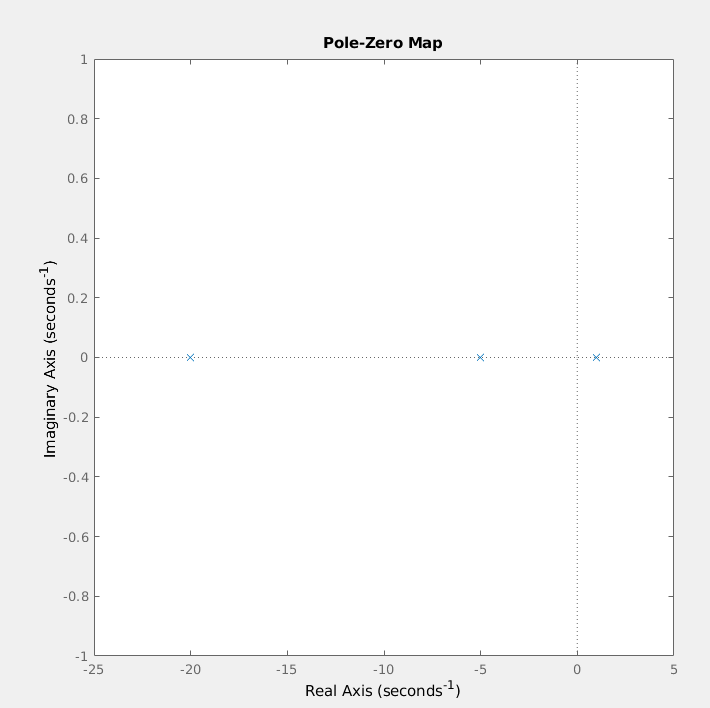
\includegraphics[width=\linewidth]{4b.png}
						\caption{Sistema inestable.}
					\end{subfigure}
					\begin{subfigure}[b]{0.49\linewidth}
						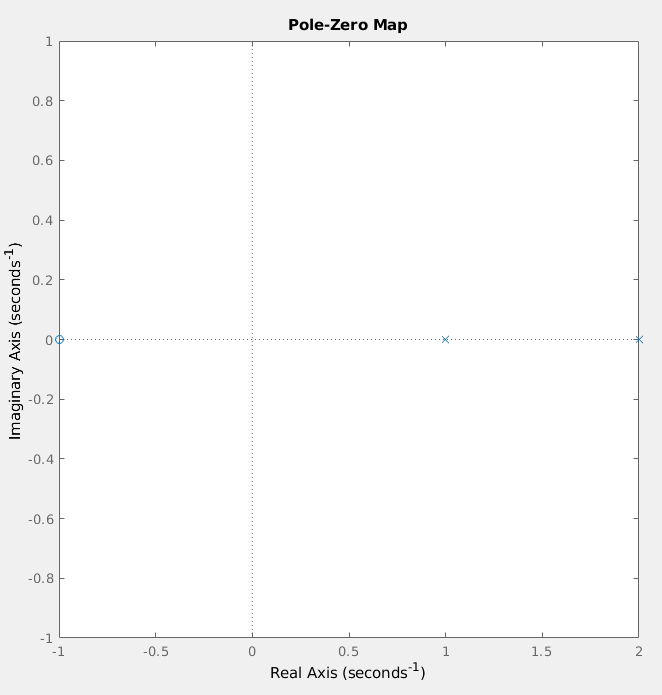
\includegraphics[width=\linewidth]{4c.png}
						\caption{Sistema inestable.}
					\end{subfigure}
					\caption{Gráficas de los polinomios y sus raíces en el plano complejo. Al igual que en ejercicio anterior, nos basamos en las mismas observaciones para determinar la estabilidad de los sistemas.}
				\end{figure}
\end{enumerate}
\section*{Conclusión}

Los controladores vistos en esta práctica son de gran ayuda en la industria debido a que, como hemos dico anteriormente, son muy sencillos de implementar y son de los más utilizados debido a esta características. Es muy fácil controlar sistemas lineales a través de ellos y si se sintonizan de manera adecuada pueden brindarnos un error muy mínimo.
%%%%%  Bib
\renewcommand\refname{Referencias}
\printbibliography
\end{document}
